% Solution: Tadelis (2013) Exercise 8.11 "Resident Assistant Selection with a Twist".
% Input by \solitem. New in the 50-item list. Check: check_D.py.
\begin{exsol}{Tadelis Exercise 8.11}{172--173}{Exam}{3}
\asked (a) The game tree of the two-veto procedure with payoffs 2/1/0; (b) the SPE and whether it
is unique; (c) Nash equilibria that are not subgame perfect; (d) whether player~2 would use a
pre-game e-mail to remove a candidate, and which one.

\method Backward induction in a finite game of perfect information (Tadelis \S8.1, Def.~8.1 and
Prop.~8.1, pp.~152--153). Every decision node starts a subgame, so the SPE are exactly the
backward-induction profiles (Def.~8.3, p.~157, and the Fact on p.~158). Nash equilibria through the
normal form of the tree (\S7.2.3, p.~143) and the on/off-path distinction (Def.~7.8, p.~146).
Lecture~4: non-credible threats, slides~8 and~13; subgames, slide~14; SPE, slide~17.

\solution
\textbf{(a) Tree.} Payoffs: $u_1(a,b,c) = (2,1,0)$ and $u_2(a,b,c) = (1,2,0)$. Player~1 vetoes one
candidate, player~2 vetoes one of the two left, and the last one is assigned. ``$\neg j$'' means
``veto $j$''; leaves show the assigned candidate and $(u_1,u_2)$.
\begin{center}
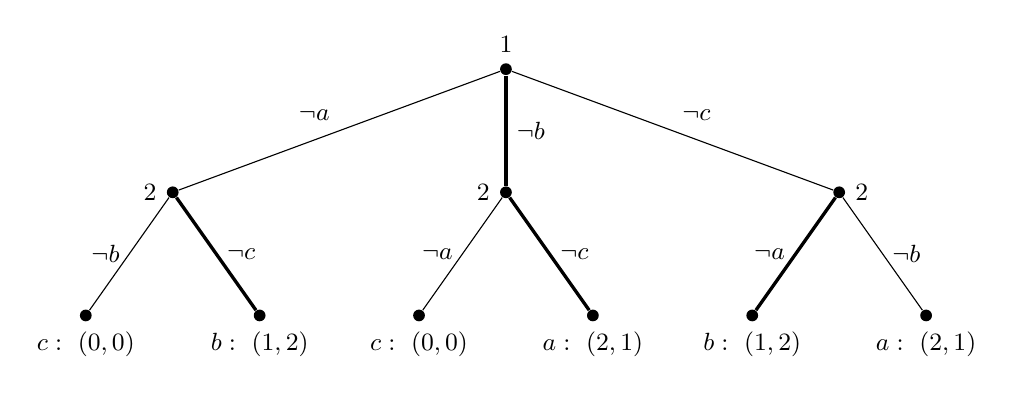
\begin{tikzpicture}[scale=0.92,dot/.style={circle,fill,inner sep=1.5pt},
  every node/.style={font=\small},t1/.style={very thick},t0/.style={}]
  \node[dot,label=above:{1}] (r) at (0,0) {};
  \node[dot,label=left:{2}] (A) at (-4.6,-1.7) {};
  \node[dot,label=left:{2}] (B) at (0,-1.7) {};
  \node[dot,label=right:{2}] (C) at (4.6,-1.7) {};
  \draw (r) -- node[above left] {$\neg a$} (A);
  \draw[very thick] (r) -- node[right] {$\neg b$} (B);
  \draw (r) -- node[above right] {$\neg c$} (C);
  \foreach \P/\x/\l/\la/\lb/\pa/\pb/\ta/\tb in
     {A/-4.6/b/{\neg b}/{\neg c}/{c:\ (0,0)}/{b:\ (1,2)}/0/1,
      B/0/a/{\neg a}/{\neg c}/{c:\ (0,0)}/{a:\ (2,1)}/0/1,
      C/4.6/a/{\neg a}/{\neg b}/{b:\ (1,2)}/{a:\ (2,1)}/1/0} {
    \node[dot,label=below:{$\pa$}] (\P1) at (\x-1.2,-3.4) {};
    \node[dot,label=below:{$\pb$}] (\P2) at (\x+1.2,-3.4) {};
    \draw[t\ta] (\P) -- node[left] {$\la$} (\P1);
    \draw[t\tb] (\P) -- node[right] {$\lb$} (\P2);}
\end{tikzpicture}\\[2pt]
{\footnotesize Thick branches = backward-induction choices.}
\end{center}
Player~1 has 3 pure strategies. Player~2 has $2^3 = 8$: write $s_2 = (x_a, x_b, x_c)$, where $x_j$ is the
candidate she vetoes after player~1 vetoed $j$.

\textbf{(b) Backward induction.} Player~2's three nodes:
\begin{itemize}
  \item after $\neg a$ ($\{b,c\}$ left): $\neg c$ leaves $b$, $u_2 = 2 > 0$, so $x_a = c$;
  \item after $\neg b$ ($\{a,c\}$ left): $\neg c$ leaves $a$, $u_2 = 1 > 0$, so $x_b = c$;
  \item after $\neg c$ ($\{a,b\}$ left): $\neg a$ leaves $b$, $u_2 = 2 > 1$, so $x_c = a$.
\end{itemize}
Player~1 anticipates the outcomes $b$, $a$, $b$ of $\neg a$, $\neg b$, $\neg c$, worth $1, 2, 1$ to
him, and vetoes $b$. The SPE is
\[
  \bigl(\ \neg b,\ \ s_2 = (c,\ c,\ a)\ \bigr), \qquad \text{outcome } a, \quad (u_1,u_2) = (2,1).
\]
It is unique: every comparison above is strict, so backward induction never has to break a tie. Player~1 vetoes
the rival's favourite, $b$, not his own least preferred, $c$. Player~2 will veto $c$ herself, so a veto
spent on $c$ is wasted.

\textbf{(c) Nash equilibria that are not subgame perfect.} Enumerating the $3 \times 8 = 24$ pure
profiles gives 7 Nash equilibria:
\begin{center}
\begin{tabular}{llcc}
\toprule
Player 1 & Player 2 $(x_a, x_b, x_c)$ & outcome, $(u_1,u_2)$ & SPE? \\
\midrule
$\neg b$ & $(c, c, a)$ & $a$, $(2,1)$ & yes \\
$\neg b$ & $(b, c, a)$, $(c, c, b)$, $(b, c, b)$ & $a$, $(2,1)$ & no \\
$\neg a$ & $(c, a, a)$ & $b$, $(1,2)$ & no \\
$\neg c$ & $(c, a, a)$, $(b, a, a)$ & $b$, $(1,2)$ & no \\
\bottomrule
\end{tabular}
\end{center}
So yes, there are six. Two kinds:
\begin{itemize}
  \item \emph{Same outcome, different off-path plans.} Player~1 vetoes $b$ and player~2 vetoes $c$ on
  the path. Off the path she plans to veto $b$ after $\neg a$ (leaving $c$: $0$ instead of $2$) or $b$
  after $\neg c$ (leaving $a$: $1$ instead of $2$). These nodes are never reached, so the plans cost
  her nothing, but they are not best responses in the subgames that start there.
  \item \emph{A different outcome, supported by a threat.} With $x_b = a$, player~2 announces: ``if
  you veto $b$, I veto $a$, and $c$ gets the job.'' Facing it, $\neg b$ gives player~1 $0$, so he
  vetoes $a$ or $c$ and player~2 gets her favourite $b$. The threat is not credible: after $\neg b$
  her choice is between $a$ (1) and $c$ (0), and she would veto $c$. Check of one of them,
  $(\neg c,\ (c,a,a))$: player~1 gets $1$ against $0$ from $\neg b$ and $1$ from $\neg a$;
  player~2 gets $2$, her maximum. The threatened node is off the path, so the threat is never
  tested.
\end{itemize}
No Nash equilibrium elects $c$: on the path, player~2 could always veto $c$ instead and gain.

\textbf{(d) The alienating e-mail.} Read as follows: the e-mail comes first and its effect is seen
by both. Then player~1 vetoes one of the two remaining candidates, and the last one is assigned
(player~2's veto has nothing left to act on). In each two-candidate subgame player~1 keeps his
preferred candidate:
\begin{center}
\begin{tabular}{lccc}
\toprule
Player 2's first move & candidates left & player 1 vetoes & outcome, $(u_1,u_2)$ \\
\midrule
no e-mail & $\{a,b,c\}$ & $b$ (part (b)) & $a$, $(2,1)$ \\
e-mail $a$ & $\{b,c\}$ & $c$ & $b$, $(1,2)$ \\
e-mail $b$ & $\{a,c\}$ & $c$ & $a$, $(2,1)$ \\
e-mail $c$ & $\{a,b\}$ & $b$ & $a$, $(2,1)$ \\
\bottomrule
\end{tabular}
\end{center}
Player~2 gets 2 only by e-mailing $a$, so she does. In the SPE of the extended game, she e-mails
$a$, player~1 vetoes $c$, and $b$ is assigned, $(u_1,u_2) = (1,2)$. The strategy profile also
specifies the original SPE after ``no e-mail'' and player~1's vetoes after the other two e-mails.

\interp The order of moves decides the outcome. Moving first, player~1 removes the rival's
favourite. Player~2 then cannot hurt him, because the only threat she has (``I'll leave you $c$'')
hurts her too. The e-mail works where the threat fails because it is an irreversible move made
before player~1 acts, not a promise about later behaviour. Player~2 removes $a$, her own second
choice. That looks self-defeating, but it takes away player~1's best option, and with only
$\{b,c\}$ left he prefers $b$. A smaller choice set helps the player who controls it. This is the
same commitment logic as the Brexit preparation (slide~11): an observable, sunk action changes
what the opponent can do, while announcing future vetoes changes nothing (``talk is cheap'', slide~11; non-credible threats, slide~13).

\verify \texttt{check\_D.py} builds the tree, runs backward induction (asserting no ties), enumerates
all 24 pure profiles and tests each one for Nash and for subgame perfection by definition (Nash in
every subgame). It then builds the extended game with the e-mail move and solves it backward.
Output: ``Tadelis 8.11: SPE veto b, then (bc: veto c, ac: veto c, ab: veto a), outcome a (2,1),
unique; 7 pure NE (4 with outcome a, 3 with outcome b), 6 not SPE'' and ``Tadelis 8.11 (d): player
2 e-mails candidate a; player 1 then vetoes c; outcome b (1,2)''. (In the script, node ``bc''
is player~2's node after $\neg a$, and so on.) Tadelis prints no answer.

\mistakes
\begin{itemize}
  \item Having player~1 veto his least-preferred candidate $c$. Player~2 would veto $c$ anyway; the
  useful veto removes her favourite.
  \item Writing player~2's strategy as one veto. She has three information sets, so a strategy is
  a triple, and it is the off-path entries that separate the Nash equilibria from the SPE.
  \item In (d), removing $c$ or $b$ (``remove the worst'' or ``remove the rival's favourite'' by
  analogy). Only removing $a$ changes player~1's choice.
\end{itemize}

\answer{(a) Tree above; player~1 has 3 strategies, player~2 has 8. (b) Unique SPE: player~1 vetoes
$b$; player~2 vetoes $c$ after $\neg a$, $c$ after $\neg b$, $a$ after $\neg c$; $a$ is
selected, payoffs $(2,1)$. (c) Yes: 7 pure Nash equilibria, 6 not subgame perfect. Three of them
elect $b$, payoffs $(1,2)$, using player~2's non-credible threat to veto $a$ after $\neg b$. (d) Yes:
she e-mails $a$; player~1 then vetoes $c$ and $b$ is selected, payoffs $(1,2)$.}
\end{exsol}
